\documentclass[a4paper,12pt]{article}
\usepackage[T1]{fontenc}
\usepackage{inputenc}
\usepackage{fontspec}
\usepackage{lmodern}
\usepackage[english]{babel}
\usepackage{hyperref}
\usepackage{float}
\usepackage{tikz} % pour la définition de couleur
\usepackage{soul} % pour surligner le texte

\usepackage[margin=2.3cm]{geometry} % marges

% MISE EN FORME DES BLOCS DE CODE
\usepackage{listings} % pour les blocs de code

\definecolor{whitegray}{gray}{0.97}
\definecolor{pearlgray}{gray}{0.94}
\definecolor{lightgray}{gray}{0.90}
\definecolor{darkgray}{gray}{0.50}
\definecolor{green}{rgb}{0.22, 0.73, 0.56}
\definecolor{red}{rgb}{0.8, 0.25, 0.33}
\definecolor{blue}{rgb}{0.36, 0.62, 0.92}
\definecolor{bluegray}{rgb}{0.33, 0.41, 0.47}

% Pour que le texte en police console soit surligné en gris clair
\let\OldTexttt\texttt
\sethlcolor{pearlgray}
\renewcommand{\texttt}[1]{\OldTexttt{\hl{#1}}}

% Pour la colorisation des nombres dans le code seulement quand il ne font pas partie de chaine de caractères ou commentaire
\newcommand\digitstyle{\color{blue}}
\makeatletter
\newcommand{\ProcessDigit}[1]
{%
	\ifnum\lst@mode=\lst@Pmode\relax%
	{\digitstyle #1}%
	\else
	#1%
	\fi
}

% Definition de l'apparence des blocs de code
\lstset{
	language=php, % définition du langage (php et javascript ont des syntaxes proches)
	basicstyle=\scriptsize\ttfamily, % petite taille, police de console
	stringstyle=\color{red}, % chaine de caractères
	backgroundcolor=\color{whitegray}, % fond
	commentstyle=\color{darkgray}\textit, % commentaires
	numberstyle=\tiny\color{darkgray}, % numero de ligne
	rulecolor=\color{lightgray}, % bordure
	keywordstyle=\color{green}\textbf, % opérateurs logiques etc
	literate=
	{0}{{{\ProcessDigit{0}}}}1
	{1}{{{\ProcessDigit{1}}}}1
	{2}{{{\ProcessDigit{2}}}}1
	{3}{{{\ProcessDigit{3}}}}1
	{4}{{{\ProcessDigit{4}}}}1
	{5}{{{\ProcessDigit{5}}}}1
	{6}{{{\ProcessDigit{6}}}}1
	{7}{{{\ProcessDigit{7}}}}1
	{8}{{{\ProcessDigit{8}}}}1
	{9}{{{\ProcessDigit{9}}}}1
	{<=}{{\(\leq\)}}1,
	morestring=[b]",
	morestring=[b]',
	morecomment=[l]//,
	aboveskip=3mm,
	belowskip=-2mm,
	breakatwhitespace=false,
	breaklines=true,
	captionpos=b,
	deletekeywords={...},
	escapeinside={\%*}{*)},
	extendedchars=true,
	framexleftmargin=16pt,
	framextopmargin=5pt,
	framexbottommargin=5pt,
	frame=tblr,
	keepspaces=true,
	morekeywords={*,...},
	numbers=left,
	numbersep=10pt,
	showspaces=false,
	showstringspaces=false,
	showtabs=false,
	stepnumber=1,
	tabsize=4,
	title=\lstname,
}

\begin{document}
\section{AmCharts V4}\label{amcharts-v4}

This page is a general introduction to the charts javascript library AmCharts in its version V4. An extensive documentaion and API can be found \href{https://www.amcharts.com/docs/v4/}{here}, demos of all the charts that can be made can be found \href{https://www.amcharts.com/demos/}{here} and tips to customize chart can be found \href{https://www.amcharts.com/t/tips/}{there}.

		\subsection{Instantiating a chart}\label{instantiating-a-chart}

			\subsubsection{Modules}\label{modules}

AmCharts allows to create several kind of charts. Depending on the one you wish to create, you will need to import several modules from the library. In all cases, you will need the main module \texttt{am4core} (which should always comes first) and an other module corresponding to the type of chart~: either the \texttt{am4charts} for all the \emph{regular} charts, or \texttt{am4maps} for map visualisations.

Some kind of charts requires additionnal plugins like force-directed graphs (\texttt{forceDirected}) or maps that need to import some geodata to display a background map (\texttt{worldLow}).

On top of that, you can import modules for \href{https://www.amcharts.com/docs/v4/getting-started/using-javascript/\#Assets}{setting assets} like translations or themes that will define behaviors and color set of the charts.

\begin{lstlisting}
<script src="https://www.amcharts.com/lib/4/core.js"></script>
<script src="https://www.amcharts.com/lib/4/charts.js"></script>
<script src="https://www.amcharts.com/lib/4/maps.js"></script>
<script src="https://www.amcharts.com/lib/4/geodata/worldLow.js"></script>
<script src="https://www.amcharts.com/lib/4/themes/animated.js"></script>
\end{lstlisting}

			\subsubsection{Creating a chart}\label{creating-a-chart}

The \texttt{create()} function is always first used to add new instances to your HTML page. It takes two arguments~:

\begin{itemize}
	\item The \textbf{tag id} of the \texttt{html} element in which is going to contain the chart (the element must already exist in your DOM, the function will not create it)~;
	\item The \textbf{type of chart}, \emph{i.e.} the class reference.
\end{itemize}

\begin{lstlisting}
var chart = am4core.create("chartdiv", am4charts.XYChart);
\end{lstlisting}

				\paragraph{Combining multiple charts}\label{combining-multiple-charts}

Is it possible to put several charts in the same \texttt{html} element. To do that you only need to create first a \href{https://www.amcharts.com/docs/v4/concepts/svg-engine/containers/}{container} in which you will create charts instances~:

\begin{lstlisting}
var container = am4core.create("chartdiv", am4core.Container);
var mapChart = container.createChild(am4maps.MapChart);
var XYChart = mapChart.chartContainer.createChild(am4charts.XYChart);
\end{lstlisting}

				\paragraph{Configuration~: object/JSON approachs}\label{configuration-objectjson-approachs}

There are two way of setting up the parameters and data for the charts~: either a \href{https://www.amcharts.com/docs/v4/getting-started/basics/\#Using_JSON}{\textbf{JSON-based}} approach, or an \href{https://www.amcharts.com/docs/v4/getting-started/basics/\#Object_based_approach}{\textbf{object-based}} approach. Object approach is more readable and less prone to bug whereas JSON approach, being fundamentally a string, can be stored in a database or load dynamically with AJAX.

The rest of this introduction will only give examples with the object approach but you can find more information \href{https://www.amcharts.com/docs/v4/concepts/json-config/}{here} on the JSON way. Object-based only means that the chart is treated as an object whose properties we're going to change/call.

		\subsection{Anatomy of a chart}\label{anatomy-of-a-chart}

A chart is mainly composed of two elements~: the \textbf{``\emph{frame}''} and the ``\textbf{\emph{shapes}}'' representing the data~:

\begin{itemize}
	\item The \emph{frame} is, in most cases, composed of two \texttt{axes} defining the structure of the chart.
	\item The data can be displayed in different \emph{shapes} depending of the type of chart~: columns, bubbles, points, line, etc. Whatever its shape, data is an instance of one or several \texttt{series}.
\end{itemize}

			\subsubsection{\href{https://www.amcharts.com/docs/v4/concepts/axes/}{Axes}}\label{axes}

Axes are the structure of the chart~; they are specially fundamental to XYChart and some other type of charts. The axes determines how the data is going to be spread out through out the chart.

The axes can be of mainly two types~:

\begin{itemize}
	\item \href{https://www.amcharts.com/docs/v4/concepts/axes/category-axis/}{\textbf{Category axis}}~: used to position data items on text-based categories. For example, for a dataset detailling the number of folio per manuscript, the category axis would represent all the manuscripts.
	\item \href{https://www.amcharts.com/docs/v4/concepts/axes/value-axis/}{\textbf{Value axis}}~: used to position data items on a numeric scale. In our previous example, it would represent the total number of folios.
	\item Other types of axes~:
	\begin{itemize}
		\item \textbf{Duration axis}
		\item \textbf{Date axis}
	\end{itemize}
\end{itemize}

And, in the case of XYCharts, axes can be horizontal -- or circular in case of some charts like radar -- (\texttt{xAxes}) or vertical (\texttt{yAxes})~; any of them can be a category axis or value axis, and both of them can be of the same type.

				\paragraph{Creating axes}\label{creating-axes}

To associate axis to a chart, you need to push them to your existing chart like so~:

\begin{lstlisting}
var valueAxis = chart.yAxes.push(new am4charts.ValueAxis());
var categoryAxis = chart.xAxes.push(new am4charts.CategoryAxis());
\end{lstlisting}

				\paragraph{Configuring axes}\label{configuring-axes}

Most of the appearence parameters and settings can be configured \href{https://www.amcharts.com/docs/v4/reference/axis/}{directly on the axis variable} or with the \href{https://www.amcharts.com/docs/v4/reference/axisrenderer/}{\texttt{renderer} property}~:

\begin{lstlisting}
// define a title for the value axis
valueAxis.title.text = "Number of folios";
// display the axis one the opposite side than the default one
categoryAxis.renderer.opposite = true;
// to set the background grid of the value axis to be transparent
valueAxis.renderer.grid.template.strokeOpacity = 0;
// set the font size of the label from the category axis to 20
categoryAxis.renderer.labels.template.fontSize = 20;
\end{lstlisting}

			\subsubsection{\href{https://www.amcharts.com/docs/v4/concepts/series/}{Series}}\label{series}

A series is a collection of similar, logically grouped data points, it gathers the configuration defining how the data is going to be displayed.

One series aggregates data you want to have the same properties. Sometimes one series will be enough to display gigantic datasets, but sometimes you will need to provide each data its series in order to specify finely the settings for each one in particular. A series, in a column chart for instance, can be either --- depending on what you want to show --- a group of columns, a single column, a group of cells through out the columns or a single cell.

Each type of chart allows only certain kind of series~: a \texttt{pieSeries} on a \texttt{mapChart} will never be displayed.

Series have two main purposes: - Setting appearance and behavior of a collection of chart items~; - Binding individual chart items to source data.

				\paragraph{Creating series}\label{creating-series}

To create a new series for your chart, you must proceed as for the axes~:

\begin{lstlisting}
var series = chart.series.push(new am4charts.ColumnSeries());
\end{lstlisting}

				\paragraph{Configuring series}\label{configuring-series}

You can set configuration for a series either \href{https://www.amcharts.com/docs/v4/reference/series/}{directly} on the series variable or through its \href{https://www.amcharts.com/docs/v4/concepts/series/\#Templates}{\texttt{template} property} (more on templates \href{https://gitlab.obspm.fr/gtopalian/DISHAS/wikis/AmCharts/developper_general_introduction\#templates}{later on})~:

\begin{lstlisting}
// setting width of the stroke
series.strokeWidth = 0;
// setting text appearing when hovering on columns
series.columns.template.tooltipText = "Number of folios in manuscript";
\end{lstlisting}

			\subsubsection{Additionnal components}\label{additionnal-components}

Inside a chart, you can add several type components like \textbf{SVG shapes}, \textbf{labels}, etc. To create them, you need to push them in your chart container, then you can configure them as you like~:

\begin{lstlisting}
var rectangle = chart.chartContainer.createChild(am4core.Container);
var rectLabel = rectangle.createChild(am4core.Label);
\end{lstlisting}

		\subsection{Data}\label{data}

			\subsubsection{\href{https://www.amcharts.com/docs/v4/concepts/data/\#Structure_of_data}{Data structure}}\label{data-structure}

All data, in order to be used by your chart, need it to be formatted as an \textbf{array of objects}~:

\begin{lstlisting}
var msData = [
  {
    "ms": "Latin 10264",
    "folios": 3
  },{
    "ms": "Bav. Lat. 1374",
    "folios": 14
  }
]
\end{lstlisting}

			\subsubsection{\href{https://www.amcharts.com/docs/v4/concepts/series/\#Binding_to_data}{Binding data}}\label{binding-data}

In order to make your chart use your data, you first need to associate your array to the data property of your chart~:

\begin{lstlisting}
chart.data = msData;
\end{lstlisting}

With this line, when we will set data properties to our chart series, it will know automatically where to find the information it needs. You can also bind a dataset to a \href{https://www.amcharts.com/docs/v4/concepts/data/\#Series_specific_data}{specific series} for complex layouts.

			\subsubsection{Using \href{https://www.amcharts.com/docs/v4/concepts/data/\#Data_fields}{\texttt{dataFields}}}\label{using-datafields}

Now, the axes and the series that have been earlier create needs to be associated with the data from our array. The \texttt{dataFields} property is a simple object that binds specific field in series, to a data field in data objects~: using \texttt{dataField} the series, as well as the category axis, will know what key in the dataset they are binded to.

\begin{lstlisting}
series.dataFields.categoryX = "ms";
series.dataFields.valueY = "folios";
categoryAxis.dataFields.category = "ms";
\end{lstlisting}

What those lines means is~: for each object in the array of data, the numerical value for the series will be found to the ``folios'' key and the string-based value will be found to the ``ms'' key. The value axis will generate itself according to the maximal value associated with the series to display, but the category axis needs to know which labels to show.

\textbf{NB}~: for each kind of chart, the syntax might vary. You will find more details on that in the numerous examples in the \href{https://www.amcharts.com/demos/}{demos}.

				\subsubsection{Using \href{https://www.amcharts.com/docs/v4/concepts/data/\#Property_fields}{\texttt{propertiesFields}}}\label{using-propertiesfields}

The \texttt{dataFields} property only holds information that is needed for the chart to be displayed, additionnal information can be binded to the chart to customize it further~: \texttt{propertyFields} are the way to tie chart element's properties to data.

Let's say some fields were added to your dataset like that~:

\begin{lstlisting}
var msData = [
  {
    "ms": "Latin 10264",
    "folios": 3,
    "color": "#fcba03",
    "url": "https://archivesetmanuscrits.bnf.fr/ark:/12148/cc71999k"
  },{
    "ms": "Bav. Lat. 1374",
    "folios": 14,
    "color": "#fc3103",
    "url": "https://digi.ub.uni-heidelberg.de/diglit/bav_pal_lat_1374"
  }
];
\end{lstlisting}

Pretty much any part of your chart can be customize using information from your dataset with the \texttt{propertiesField} property~:

\begin{lstlisting}
// make column labels a link
categoryAxis.renderer.labels.template.propertyFields.url = "url";
// colour the columns
series.columns.template.propertyFields.fill = "color";
\end{lstlisting}

				\paragraph{Using \href{https://www.amcharts.com/docs/v4/concepts/data/\#Using_dummy_data_}{\texttt{dummyData}}}\label{using-dummydata}

You can bind any data of your choice to a chart item using its \texttt{dummyData} property~: it is a sort of storage container to put anything you want in it, without affecting the overall behavior of your chart.

It can be very useful when you will need to customize your chart creating tailored function using \href{https://www.amcharts.com/docs/v4/concepts/event-listeners/}{event listeners} or \href{https://www.amcharts.com/docs/v4/concepts/adapters/}{adapters}~: it can become handy if you are dynamically generating data you want to access later on, for instance to bind behavior for two distinct events.

		\subsection{Appearance configuration}\label{appearance-configuration}

			\subsubsection{\href{https://www.amcharts.com/docs/v4/concepts/list-templates/}{Templates}}\label{templates}

Practically all of the charts components have a \texttt{template} property~: it is some kind of pattern for the layout and behavior of specific parts of your chart. Using templates, you can, for example, set that all filling colors of columns to be half transparent or for all axis labels to become green when clicked on~:

\begin{lstlisting}
// Half transparency of the columns
series.columns.template.fillOpacity = 0.5;
// Green labels
valueAxis.renderer.labels.template.events.on("hit", function(ev) {
  valueAxis.renderer.labels.template.fill = "green";
});
\end{lstlisting}

Templates can be modified dynamically using DOM events, which is not the case with data values (associated with \texttt{dataFields})~: to change the values your chart is using, you will need either to \href{https://codepen.io/segolene-albouy/pen/rExamo}{switch datasets} or use \href{https://www.amcharts.com/docs/v4/concepts/data/\#Incremental_updates}{incremental loading}).

AmCharts is an incredibly customisable library~: if you would like to change any aspects of your chart, by browsing through the properties of the element you want to modify in the \href{https://www.amcharts.com/docs/v4/reference/}{API}, you will surely find something to suit your desires.

			\subsubsection{\href{https://www.amcharts.com/docs/v4/concepts/colors/}{Colors}, percentage, etc.}\label{colors-percentage-etc.}

To unlock all methods applicable to colors and percentages, you will need to use special Amcharts functions. The \texttt{color()} method takes only one argument of color and transform it into an object that can be later on \href{https://www.amcharts.com/docs/v4/reference/color/\#Methods}{modified}. The same is true for \href{https://www.amcharts.com/docs/v4/reference/percent/}{\texttt{percent()}} method. To define the color or the percentage of a property~:

\begin{lstlisting}
rectangle.width = am4core.percent(50);
rectangle.background.fill = am4core.color("orange");
\end{lstlisting}

				\paragraph{\href{https://www.amcharts.com/docs/v4/concepts/series/\#Defining_a_heat_rule}{Heat rules}}\label{heat-rules}

Heat rules defines a property of a chart item that will be bind to a numeric value. Any property is usable, as long as you can define a min and max state like so~:

\begin{lstlisting}
// The higher the value, the wider the column
series.heatRules.push({
    target: series.columns.template,
    property: "width",
    min: 80,
    max: 160
});
\end{lstlisting}

			\subsubsection{\href{https://www.amcharts.com/docs/v4/concepts/states/}{States}}\label{states}

Any part of the chart can be associated with a \texttt{state} object that holds properties defining how the element will behave when on this particular state. States define alternative properties that will override ``\emph{normal state}'' properties on certain occasions.

As many other objects in AmCharts, defining state is a two steps process~: first \textbf{creating} the state for a specific element, then \textbf{configurating} it~:

\begin{lstlisting}
var hoverState = series.columns.template.states.create("hover");
hoverState.properties.fillOpacity = 0.9;
\end{lstlisting}

			\subsubsection{\href{https://www.amcharts.com/docs/v4/concepts/formatters/formatting-strings/}{Formatting text} in labels and tooltips}\label{formatting-text-in-labels-and-tooltips}

				\paragraph{\href{https://www.amcharts.com/docs/v4/concepts/formatters/formatting-strings/\#Visual_formatting}{Font styling}}\label{font-styling}

Text styling options are always contained in \texttt{{[}square brackets{]}}. It works like HTML tag so each opening bracket should be closed with a closing bracket (\texttt{{[}/{]}}), but an other opening bracket will act as a closing one for one opened earlier.

Some styling have an already \href{https://www.amcharts.com/docs/v4/concepts/formatters/formatting-strings/\#Visual_formatting}{implemented syntax} in AmCharts, but you can use any CSS property~:

\begin{lstlisting}
rectLabel.text = "[bold]Work diffusion[/] :\n the example of the [font-style: italic]Tabule Magne[/]";
\end{lstlisting}

				\paragraph{Accessing \href{https://www.amcharts.com/docs/v4/concepts/data/\#Placeholders_in_on_screen_text}{data values}}\label{accessing-data-values}

Is it possible to display data in labels with the \texttt{\{curly brackets\}} notation. Depending on \href{https://www.amcharts.com/docs/v4/concepts/formatters/formatting-strings/\#Placeholder_examples}{what you write} in your brackets, the parser (or the ``formatter'' to use AmCharts taxonomy) will try to find matching data in your dataset. You can either use the name of a key in your dataset, or the class reference of the data~:

\begin{lstlisting}
series.columns.template.tooltipText = "Numbers of [{color}]folios[/] in {ms} : \n {valueY}";
\end{lstlisting}

You can even perform some data computing on your numeric values with the formatter using \href{https://www.amcharts.com/docs/v4/concepts/formatters/formatting-strings/\#Placeholders_for_numeric_values}{modifiers} such as \texttt{sum} or \texttt{count}.

				\paragraph{Using HTML}\label{using-html}

You can also display any HTML elements in your \href{https://www.amcharts.com/docs/v4/tutorials/tooltips-with-rich-html-content/}{tooltips} and \href{https://www.amcharts.com/docs/v4/reference/label/\#html_property}{labels} using the \texttt{html} or \texttt{tooltipHTML} property :

\begin{lstlisting}
rectangle.tooltipHTML = '<span style="font-variant: small-caps;">Regarding folio quantity in manuscript</span>';
\end{lstlisting}

		\subsection{Additionnal features}\label{additionnal-features}

Satellite elements can be instantiated by creating a new object of their class, they will behave accordingly to their normal use but you can completely divert their utility

			\subsubsection{\href{https://www.amcharts.com/docs/v4/concepts/chart-cursor/}{Cursors}}\label{cursors}

Cursors are only available for XY charts and radar charts~: they allow to add interactivity to charts as well as providing zoom modalities.

\begin{lstlisting}
chart.cursor = new am4charts.XYCursor();
\end{lstlisting}

By default, cursors, when moving on the chart, display two crossing lines ending with tooltips to better pinpoint and understand the data, but all of this can be disabled or modified. You can as well, add some cursor behaviors to allow \href{https://www.amcharts.com/docs/v4/concepts/chart-cursor/\#Zooming_panning}{zooming and panning}~:

\begin{lstlisting}
chart.cursor.behavior = "selectX";
\end{lstlisting}

			\subsubsection{\href{https://www.amcharts.com/docs/v4/reference/scrollbar/}{Scrollbar}}\label{scrollbar}

A scrollbar is associated to an axis of the chart and allows to zoom in it. Is it possible to push series in it to display a \href{https://www.amcharts.com/docs/v4/chart-types/xy-chart/\#Scrollbar_with_preview}{preview} of the value of your chart, even to \href{https://www.amcharts.com/docs/v4/tutorials/scrollbar-only-xy-chart/}{treat it as a chart} in itself.

\begin{lstlisting}
var scrollbarX = new am4charts.XYChartScrollbar();
scrollbarX.series.push(series);
chart.scrollbarX = scrollbarX;
\end{lstlisting}

			\subsubsection{\href{https://www.amcharts.com/docs/v4/concepts/legend/}{Legends}}\label{legends}

A legend, when created, will automatically display the series that are associated to your chart. When clicking of the items of the legend, corresponding series disappear, giving possibilities to vary the visualization to the user.

In the case of our manuscript chart, adding a legend is not very insightful, because our data is contained in an unique series representing all the columns, which colors were assigned individually. If we wanted to display a matching legend, we would need to build a \href{https://www.amcharts.com/docs/v4/concepts/legend/\#Adding_custom_items}{custom legend}.

\begin{lstlisting}
chart.legend = new am4charts.Legend();
\end{lstlisting}

			\subsubsection{\href{https://www.amcharts.com/docs/v4/concepts/event-listeners/}{Events listeners}}\label{events-listeners}

Event listeners allows to bind custom functions to any action perform on a chart element. Each part of the chart has a list of events tied to variables that can be accessed and modified when the event is triggered.

Two kind of functions can be associated to the events~:
\begin{itemize}
	\item \texttt{on()}~: any time the event happens~;
	\item \texttt{once()}~: the first time the event happens.s
\end{itemize}

\begin{lstlisting}
chart.cursor.events.on("selectended", function(ev) {
  var range = ev.target.xRange;
  var axis = ev.target.chart.xAxes.getIndex(0);
  var from = axis.getPositionLabel(axis.toAxisPosition(range.start));
  var to = axis.getPositionLabel(axis.toAxisPosition(range.end));
  alert("Selected from " + from + " to " + to);
});
\end{lstlisting}

The syntax for setting custom functions is always the same~:

\texttt{\{chartName\}.\{elementName\}.events.{[}on/once{]}("\{eventName\}", function(args) \{...\});}

Some events are universal to any type of element, as \texttt{hit}, when the user is clicking or tapping on a touch screen.

		\subsection{Demos}\label{demos}

			\subsubsection{Our manuscript chart}\label{our-manuscript-chart}

Here is the chart that was made during this introduction : \href{https://codepen.io/segolene-albouy/pen/LwRBdg}{Number of folios in manuscript}.

\begin{figure}[H]
	\centering
	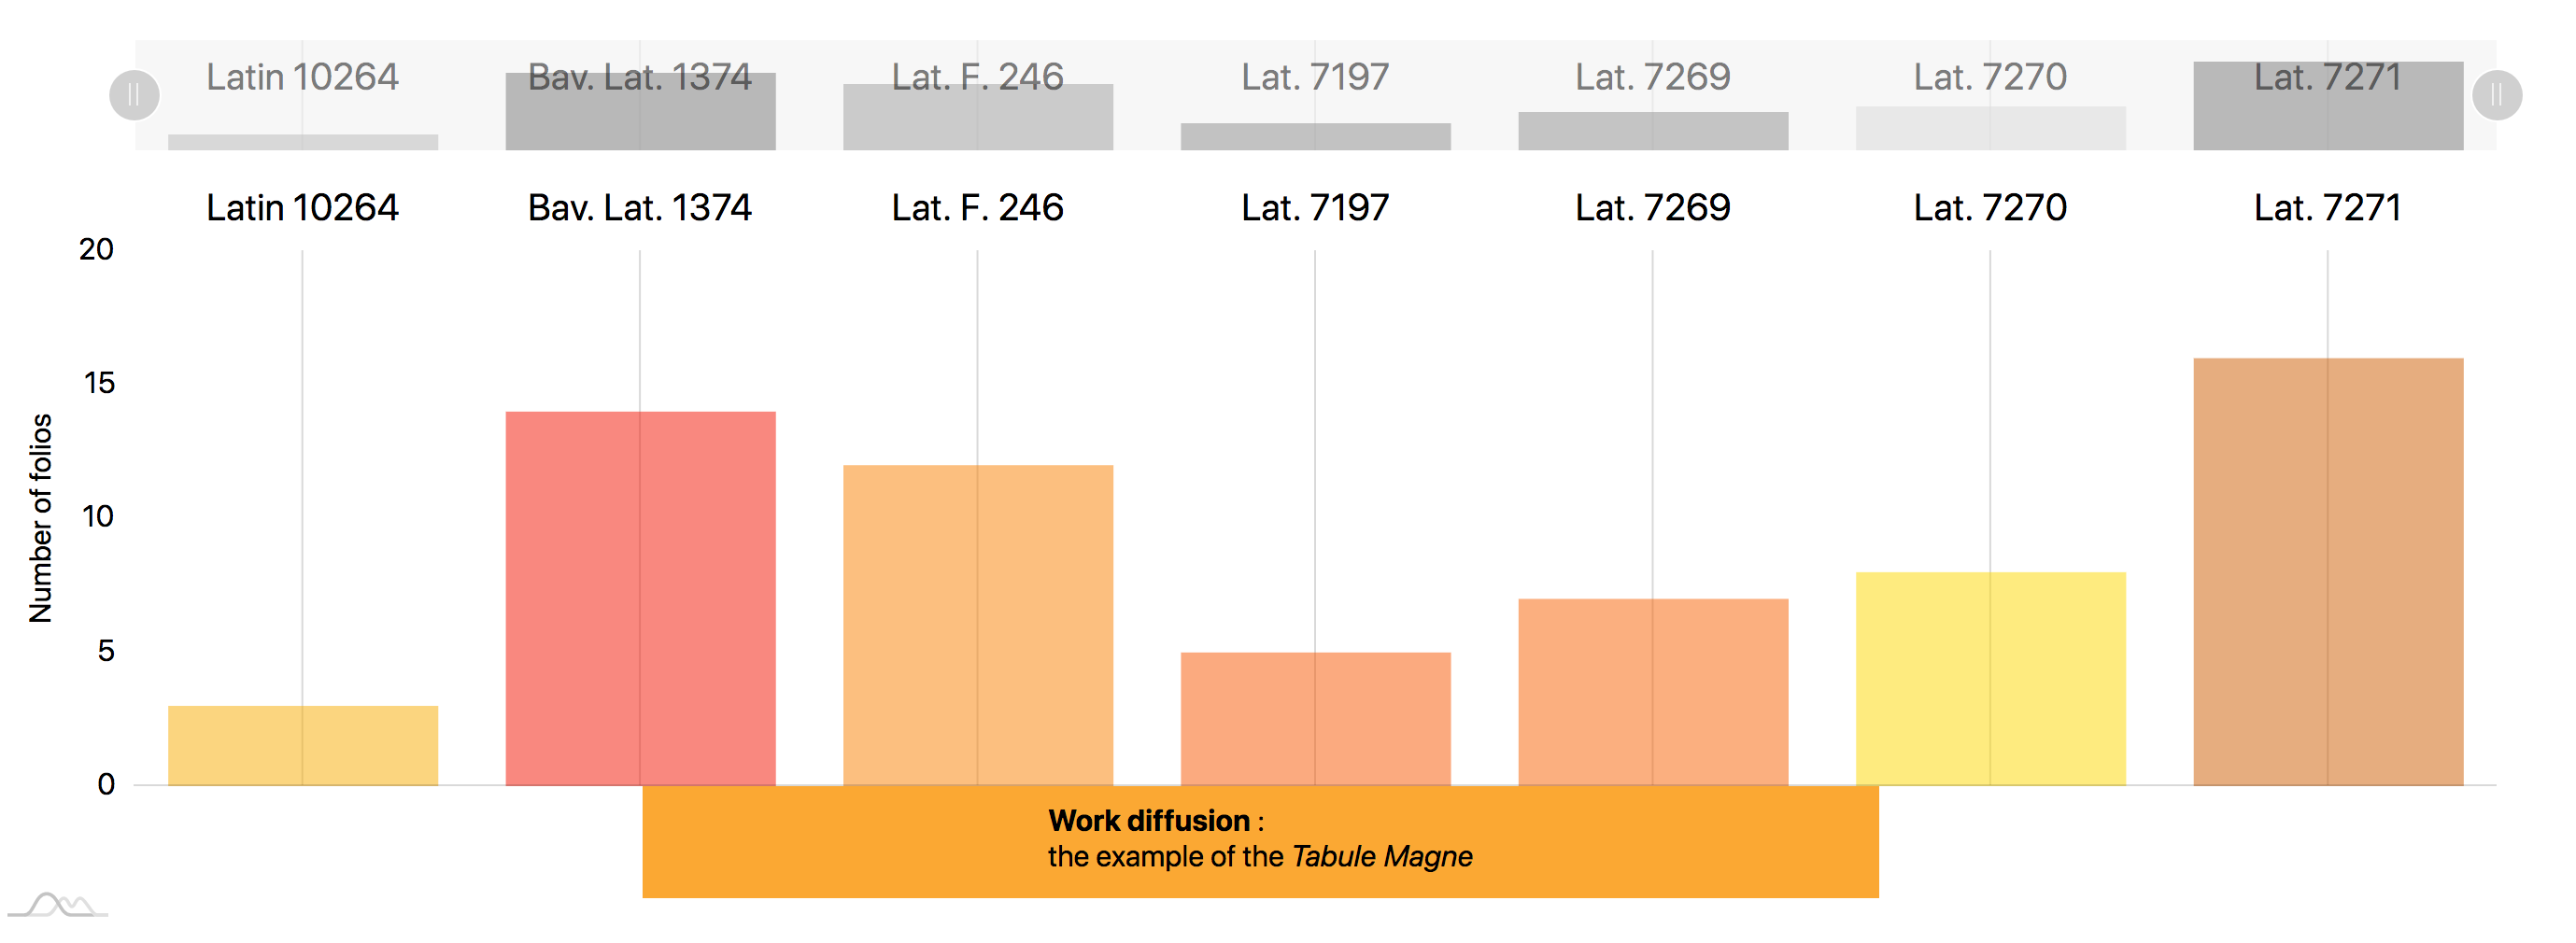
\includegraphics[width=15cm]{../../Images/Visualisations/Chart-tutoriel.png}
	\caption{Chart made during the AmCharts tutorial}
\end{figure}

			\subsubsection{Examples in DISHAS}\label{examples-in-dishas}

\begin{itemize}
	\item Primary source~: \href{https://codepen.io/segolene-albouy/pen/rExamo}{dynamic bar chart}
	\item Historical sources~: \href{https://codepen.io/segolene-albouy/pen/KOKBwL}{historical map}
\end{itemize}

\end{document}